
%%--------------------------------------------------
%% Halliday: Fundamentals of Physics
%%--------------------------------------------------


%% Chapter 02: Motion Along a Straight Line
%%--------------------------------------------------


%% Learning Objectives
%%--------------------------------------------------

%% 2.01: Identify that if all parts of an object move in the same direction and at the same rate, we can treat the object as if it were a (point-like) particle. 
%%      (This chapter is about the motion of such objects.)
%% 2.02: Identify that the position of a particle is its location as read on a scaled axis, such as an x axis.
%% 2.03: Apply the relationship between a particle's displacement and its initial and final positions.
%% 2.04: Apply the relationship between a particle’s average velocity, its displacement, and the time interval for that displacement.
%% 2.05: Apply the relationship between a particle’s average speed, the total distance it moves, and the time interval for the motion.
%% 2.06: Given a graph of a particle’s position versus time, determine the average velocity between any two particular times.


%% Halliday Multiple Choice Questions
%%--------------------------------------------------
\element{halliday-mc}{
\begin{question}{halliday-ch02-q01}
    A particle moves along the $x$ axis from $x_i$ to $x_f$. 
    Of the following values of the initial and final coordinates,
        which results in the displacement with the largest magnitude?
    \begin{choices}
        \wrongchoice{$x_i=\SI{4}{\meter}$,   $x_f=\SI{6}{\meter}$}
        \wrongchoice{$x_i=\SI{-4}{\meter}$,  $x_f=\SI{-8}{\meter}$}
        \wrongchoice{$x_i=\SI{-4}{\meter}$,  $x_f=\SI{2}{\meter}$}
        \wrongchoice{$x_i=\SI{4}{\meter}$,   $x_f=\SI{-2}{\meter}$}
      \correctchoice{$x_i=\SI{-4}{\meter}$, $x_f=\SI{4}{\meter}$}
    \end{choices}
\end{question}
}

\element{halliday-mc}{
\begin{question}{halliday-ch02-q02}
    A particle moves along the $x$ axis from $x_i$ to $x_f$. 
    Of the following values of the initial and final coordinates,
        which results in a negative displacement?
    \begin{choices}
        \wrongchoice{$x_i=\SI{4}{\meter}$,   $x_f=\SI{6}{\meter}$}
      \correctchoice{$x_i=\SI{-4}{\meter}$,  $x_f=\SI{-8}{\meter}$}
        \wrongchoice{$x_i=\SI{-4}{\meter}$,  $x_f=\SI{2}{\meter}$}
        \wrongchoice{$x_i=\SI{-4}{\meter}$,   $x_f=\SI{-2}{\meter}$}
        \wrongchoice{$x_i=\SI{-4}{\meter}$, $x_f=\SI{4}{\meter}$}
    \end{choices}
\end{question}
}

\element{halliday-mc}{
\begin{question}{halliday-ch02-q03}
    The average speed of a moving object during a given interval of time is always:
    \begin{choices}
        \wrongchoice{the magnitude of its average velocity over the interval}
      \correctchoice{the distance covered during the time interval divided by the time interval}
        \wrongchoice{one-half its speed at the end of the interval}
        \wrongchoice{its acceleration multiplied by the time interval}
        \wrongchoice{one-half its acceleration multiplied by the time interval.}
    \end{choices}
\end{question}
}

\element{halliday-mc}{
\begin{question}{halliday-ch02-q04}
    Two automobiles are \SI{150}{\kilo\meter} apart and traveling toward each other. 
    One automobile is moving at \SI{60}{\kilo\meter\per\hour} and the other is moving at \SI{40}{\kilo\meter\per\hour}.
    In how many hours will they meet?
    \begin{multicols}{3}
    \begin{choices}
        \wrongchoice{\SI{2.5}{\hour}}
        \wrongchoice{\SI{2.0}{\hour}}
        \wrongchoice{\SI{1.75}{\hour}}
      \correctchoice{\SI{1.5}{\hour}}
        \wrongchoice{\SI{1.25}{\hour}}
    \end{choices}
    \end{multicols}
\end{question}
}

\element{halliday-mc}{
\begin{question}{halliday-ch02-q05}
    A car travels \SI{40}{\kilo\meter} at an average speed of \SI{80}{\kilo\meter\per\hour} and then travels \SI{40}{\kilo\meter} at an average speed of \SI{40}{\kilo\meter\per\hour}.
    The average speed of the car for this \SI{80}{\kilo\meter} trip is:
    \begin{multicols}{3}
    \begin{choices}
        \wrongchoice{\SI{40}{\kilo\meter\per\hour}}
        \wrongchoice{\SI{45}{\kilo\meter\per\hour}}
        \wrongchoice{\SI{48}{\kilo\meter\per\hour}}
      \correctchoice{\SI{53}{\kilo\meter\per\hour}}
        \wrongchoice{\SI{80}{\kilo\meter\per\hour}}
    \end{choices}
    \end{multicols}
\end{question}
}

\element{halliday-mc}{
\begin{question}{halliday-ch02-q06}
    A car starts from Hither, goes \SI{50}{\kilo\meter} in a straight line to Yon,
        immediately turns around, and returns to Hither. 
    The time for this round trip is 2 hours. 
    The magnitude of the average velocity of the car for this round trip is:
    \begin{multicols}{2}
    \begin{choices}
      \correctchoice{zero}
        \wrongchoice{\SI{50}{\kilo\meter\per\hour}}
        \wrongchoice{\SI{100}{\kilo\meter\per\hour}}
        \wrongchoice{\SI{200}{\kilo\meter\per\hour}}
        \wrongchoice{cannot be calculated without knowing the acceleration}
    \end{choices}
    \end{multicols}
\end{question}
}

\element{halliday-mc}{
\begin{question}{halliday-ch02-q07}
    A car starts from Hither, goes \SI{50}{\kilo\meter} in a straight line to Yon,
        immediately turns around, and returns to Hither. 
    The time for this round trip is 2 hours. 
    The average speed of the car for this round trip is:
    \begin{multicols}{2}
    \begin{choices}
        \wrongchoice{zero}
      \correctchoice{\SI{50}{\kilo\meter\per\hour}}
        \wrongchoice{\SI{100}{\kilo\meter\per\hour}}
        \wrongchoice{\SI{200}{\kilo\meter\per\hour}}
        \wrongchoice{cannot be calculated without knowing the acceleration}
    \end{choices}
    \end{multicols}
\end{question}
}

\element{halliday-mc}{
\begin{question}{halliday-ch02-q08}
    The coordinate of a particle in meters is given by $x(t) = 16t - 3.0t^3$,
        where the time $t$ is in seconds. 
    The particle is momentarily at rest at $t=$
    \begin{multicols}{3}
    \begin{choices}
        \wrongchoice{\SI{0.75}{\second}}
      \correctchoice{\SI{1.3}{\second}}
        \wrongchoice{\SI{5.3}{\second}}
        \wrongchoice{\SI{7.3}{\second}}
        \wrongchoice{\SI{9.3}{\second}}
    \end{choices}
    \end{multicols}
\end{question}
}

\element{halliday-mc}{
\begin{question}{halliday-ch02-q09}
    A drag racing car starts from rest at $t=0$ and moves along a straight line with velocity given by $v = bt^2$, where $b$ is a constant.
    The expression for the distance traveled by this car from its position at $t=0$ is:
    \begin{multicols}{3}
    \begin{choices}
        \wrongchoice{$bt^3$}
      \correctchoice{$\dfrac{bt^3}{3}$}
        \wrongchoice{$4bt^2$}
        \wrongchoice{$3bt^2$}
        \wrongchoice{$\dfrac{bt^3}{2}$}
    \end{choices}
    \end{multicols}
\end{question}
}

\element{halliday-mc}{
\begin{question}{halliday-ch02-q10}
    A ball rolls up a slope. 
    At the end of three seconds its velocity is \SI{20}{\centi\meter\per\second};
        at the end of eight seconds its velocity is zero. 
    What is the average acceleration from the third to the eighth second?
    \begin{multicols}{3}
    \begin{choices}
        \wrongchoice{\SI{2.5}{\centi\meter\per\second\squared}}
      \correctchoice{\SI{4.0}{\centi\meter\per\second\squared}}
        \wrongchoice{\SI{5.0}{\centi\meter\per\second\squared}}
        \wrongchoice{\SI{6.0}{\centi\meter\per\second\squared}}
        \wrongchoice{\SI{6.67}{\centi\meter\per\second\squared}}
    \end{choices}
    \end{multicols}
\end{question}
}

\element{halliday-mc}{
\begin{question}{halliday-ch02-q11}
    The coordinate of an object is given as a function of time by $x=7t-3t^2$,
        where $x$ is in meters and $t$ is in seconds. 
    Its average velocity over the interval from $t=0$ to $t=\SI{4}{\second}$ is:
    \begin{multicols}{3}
    \begin{choices}
        \wrongchoice{\SI{5}{\meter\per\second}}
      \correctchoice{\SI{-5}{\meter\per\second}}
        \wrongchoice{\SI{11}{\meter\per\second}}
        \wrongchoice{\SI{-11}{\meter\per\second}}
        \wrongchoice{\SI{-14.5}{\meter\per\second}}
    \end{choices}
    \end{multicols}
\end{question}
}

\element{halliday-mc}{
\begin{question}{halliday-ch02-q12}
    The velocity of an object is given as a function of time by $v=4t-3t^2$,
        where $v$ is in meters per second and $t$ is in seconds. 
    Its average velocity over the interval from $t=0$ to $t=\SI{2}{\second}$:
    \begin{multicols}{2}
    \begin{choices}
      \correctchoice{is zero}
        \wrongchoice{is \SI{-2}{\meter\per\second}}
        \wrongchoice{is \SI{2}{\meter\per\second}}
        \wrongchoice{is \SI{-4}{\meter\per\second}}
        \wrongchoice{cannot be calculated unless the initial position is given}
    \end{choices}
    \end{multicols}
\end{question}
}

\element{halliday-mc}{
\begin{question}{halliday-ch02-q13}
    The coordinate of an object is given as a function of time by $x=4t^2-3t^3$,
        where $x$ is in meters and $t$ is in seconds. 
    Its average acceleration over the interval from $t=0$ to $t=\SI{2}{\second}$ is:
    \begin{multicols}{2}
    \begin{choices}
        \wrongchoice{\SI{-4}{\meter\per\second\squared}}
        \wrongchoice{\SI{4}{\meter\per\second\squared}}
      \correctchoice{\SI{-10}{\meter\per\second\squared}}
        \wrongchoice{\SI{10}{\meter\per\second\squared}}
        \wrongchoice{\SI{-13}{\meter\per\second\squared}}
    \end{choices}
    \end{multicols}
\end{question}
}

%% NOTE: changed q14 and q15 to questionmult
\element{halliday-mc}{
\begin{questionmult}{halliday-ch02-q14}
    Each of four particles move along an $x$ axis.
    Their coordinates (in meters) as functions of time (in seconds) are given.
    Which of these particles have constant acceleration?
    \begin{choices}
        \wrongchoice{$x(t) = 3.5 - 2.7t^3$}
        \wrongchoice{$x(t) = 3.5 + 2.7t^3$}
      \correctchoice{$x(t) = 3.5 + 2.7t^2$}
      \correctchoice{$x(t) = 3.5 - 3.4t - 2.7t^2$}
    \end{choices}
\end{questionmult}
}

\element{halliday-mc}{
\begin{questionmult}{halliday-ch02-q15}
    Each of four particles move along an $x$ axis. 
    Their coordinates (in meters) as functions of time (in seconds) are given.
    Which of these particles is speeding up for $t>0$?
    \begin{choices}
      \correctchoice{$x(t) = 3.5 - 2.7t^3$}
      \correctchoice{$x(t) = 3.5 + 2.7t^3$}
      \correctchoice{$x(t) = 3.5 + 2.7t^2$}
      \correctchoice{$x(t) = 3.5 - 3.4t - 2.7t^2$}
    \end{choices}
\end{questionmult}
}

\element{halliday-mc}{
\begin{question}{halliday-ch02-q16}
    An object starts from rest at the origin and moves along the $x$ axis with a constant acceleration of \SI{4}{\meter\per\second\squared}. 
    Its average velocity as it goes from $x=\SI{2}{\meter}$ to $x=\SI{8}{\meter}$ is:
    \begin{multicols}{3}
    \begin{choices}
        \wrongchoice{\SI{1}{\meter\per\second}}
        \wrongchoice{\SI{2}{\meter\per\second}}
        \wrongchoice{\SI{3}{\meter\per\second}}
        \wrongchoice{\SI{5}{\meter\per\second}}
      \correctchoice{\SI{6}{\meter\per\second}}
    \end{choices}
    \end{multicols}
\end{question}
}

\element{halliday-mc}{
\begin{question}{halliday-ch02-q17}
    Of the following situations, which one is impossible?
    \begin{choices}
        \wrongchoice{A body having velocity east and acceleration east}
        \wrongchoice{A body having velocity east and acceleration west}
        \wrongchoice{A body having zero velocity and non-zero acceleration}
        \wrongchoice{A body having constant acceleration and variable velocity}
      \correctchoice{A body having constant velocity and variable acceleration}
    \end{choices}
\end{question}
}

\element{halliday-mc}{
\begin{question}{halliday-ch02-q18}
    Throughout a time interval,
        while the speed of a particle increases as it moves along the $x$ axis,
        its velocity and acceleration might be:
    \begin{choices}
        \wrongchoice{positive and negative, respectively}
        \wrongchoice{negative and positive, respectively}
      \correctchoice{negative and negative, respectively}
        \wrongchoice{negative and zero, respectively}
        \wrongchoice{positive and zero, respectively}
    \end{choices}
\end{question}
}

% NOTE: changed q19 to questionmult
\element{halliday-mc}{
\begin{questionmult}{halliday-ch02-q19}
    A particle moves on the $x$ axis. 
    When its acceleration is positive and increasing:
    \begin{choices}
        \wrongchoice{its velocity must be positive}
        \wrongchoice{its velocity must be negative}
        \wrongchoice{it must be slowing down}
        \wrongchoice{it must be speeding up}
        %\correctchoice{none of the provided must be true}
    \end{choices}
\end{questionmult}
}

\element{halliday-mc}{
\begin{question}{halliday-ch02-q20}
    The position $y$ of a particle moving along the $y$ axis depends on the time $t$ according to the equation $y=at-bt^2$. 
    The dimensions of the quantities $a$ and $b$ are respectively:
    \begin{multicols}{2}
    \begin{choices}
        \wrongchoice{$\dfrac{\mathrm{L}^2}{T}$,          $\dfrac{\mathrm{L}^3}{\mathrm{T}^2}$}
        \wrongchoice{$\dfrac{\mathrm{L}}{\mathrm{T}^2}$, $\dfrac{\mathrm{L}^2}{\mathrm{T}}$}
      \correctchoice{$\dfrac{\mathrm{L}}{\mathrm{T}}$,    $\dfrac{\mathrm{L}}{\mathrm{T}^2}$}
        \wrongchoice{$\dfrac{\mathrm{L}^3}{\mathrm{T}}$, $\dfrac{\mathrm{T}^2}{\mathrm{L}}$}
        \wrongchoice{none of the provided}
    \end{choices}
    \end{multicols}
\end{question}
}

\element{halliday-mc}{
\begin{question}{halliday-ch02-q21}
    A particle moves along the $x$ axis according to the equation $x=6t^2$,
        where $x$ is in meters and $t$ is in seconds. 
    Therefore:
    \begin{choices}
        \wrongchoice{the acceleration of the particle is \SI{6}{\meter\per\second\squared}}
        \wrongchoice{$t$ cannot be negative}
        \wrongchoice{the particle follows a parabolic path}
        \wrongchoice{each second the velocity of the particle changes by \SI{9.8}{\meter\per\second}}
      \correctchoice{none of the provided}
    \end{choices}
\end{question}
}

\element{halliday-mc}{
\begin{question}{halliday-ch02-q22}
    Over a short interval near time $t=0$ the coordinate of an automobile in meters is given by $x(t)=27t-4.0t^3$,
        where $t$ is in seconds. 
    At the end of \SI{1.0}{\second} the acceleration of the auto is:
    \begin{multicols}{3}
    \begin{choices}
        \wrongchoice{\SI{27}{\meter\per\second\squared}}
        \wrongchoice{\SI{4.0}{\meter\per\second\squared}}
        \wrongchoice{\SI{-4.0}{\meter\per\second\squared}}
        \wrongchoice{\SI{-12}{\meter\per\second\squared}}
      \correctchoice{\SI{-24}{\meter\per\second\squared}}
    \end{choices}
    \end{multicols}
\end{question}
}

\element{halliday-mc}{
\begin{question}{halliday-ch02-q23}
    Over a short interval, starting at time $t=0$,
        the coordinate of an automobile in meters is given by $x(t)=27t-4.0t^3$,
        where $t$ is in seconds. 
    The magnitudes of the initial (at $t=0$) velocity and acceleration of the auto respectively are:
    \begin{multicols}{2}
    \begin{choices}
        \wrongchoice{zero; \SI{12}{\meter\per\second\squared}}
        \wrongchoice{zero; \SI{24}{\meter\per\second\squared}}
      \correctchoice{\SI{27}{\meter\per\second}; zero}
        \wrongchoice{\SI{27}{\meter\per\second}; \SI{12}{\meter\per\second\squared}}
        \wrongchoice{\SI{27}{\meter\per\second}; \SI{24}{\meter\per\second\squared}}
    \end{choices}
    \end{multicols}
\end{question}
}

\element{halliday-mc}{
\begin{question}{halliday-ch02-q24}
    At time $t=0$ a car has a velocity of \SI{16}{\meter\per\second}. 
    It slows down with an acceleration given by $-0.50t$,
        in \si{\meter\per\second\squared} for $t$ in seconds. 
    It stops at $t=$
    \begin{multicols}{3}
    \begin{choices}
        \wrongchoice{\SI{64}{\second}}
        \wrongchoice{\SI{32}{\second}}
        \wrongchoice{\SI{16}{\second}}
      \correctchoice{\SI{8.0}{\second}}
        \wrongchoice{\SI{4.0}{\second}}
    \end{choices}
    \end{multicols}
\end{question}
}

\element{halliday-mc}{
\begin{question}{halliday-ch02-q25}
    At time $t=0$ a car has a velocity of \SI{16}{\meter\per\second}. 
    It slows down with an acceleration given by $-0.50t$, in \si{\meter\per\second\squared} for $t$ in seconds.
    At the end of \SI{4.0}{\second} it has traveled:
    \begin{multicols}{3}
    \begin{choices}
        \wrongchoice{zero}
        \wrongchoice{\SI{12}{\meter}}
        \wrongchoice{\SI{14}{\meter}}
        \wrongchoice{\SI{25}{\meter}}
      \correctchoice{\SI{59}{\meter}}
    \end{choices}
    \end{multicols}
\end{question}
}

\element{halliday-mc}{
\begin{question}{halliday-ch02-q26}
    At time $t=0$ a car has a velocity of \SI{16}{\meter\per\second}.
    It slows down with an acceleration given by $-0.50t$, in \si{\meter\per\second\squared} for $t$ in seconds.
    By the time it stops it has traveled:
    \begin{multicols}{3}
    \begin{choices}
        \wrongchoice{\SI{15}{\meter}}
        \wrongchoice{\SI{31}{\meter}}
        \wrongchoice{\SI{62}{\meter}}
      \correctchoice{\SI{85}{\meter}}
        \wrongchoice{\SI{100}{\meter}}
    \end{choices}
    \end{multicols}
\end{question}
}

\element{halliday-mc}{
\begin{question}{halliday-ch02-q27}
    Starting at time $t=0$,
        an object moves along a straight line with velocity in \si{\meter\per\second} given by $v(t)=98-2t^2$,
        where $t$ is in seconds. 
    When it momentarily stops its acceleration is:
    \begin{multicols}{3}
    \begin{choices}
        \wrongchoice{zero}
        \wrongchoice{\SI{-4.0}{\meter\per\second\squared}}
        \wrongchoice{\SI{-9.8}{\meter\per\second\squared}}
      \correctchoice{\SI{-28}{\meter\per\second\squared}}
        \wrongchoice{\SI{49}{\meter\per\second\squared}}
    \end{choices}
    \end{multicols}
\end{question}
}

\element{halliday-mc}{
\begin{question}{halliday-ch02-q28}
    Starting at time $t=0$, an object moves along a straight line. 
    Its coordinate in meters is given by $x(t)=75t-1.0t^3$,
        where $t$ is in seconds. 
    When it momentarily stops its acceleration is:
    \begin{multicols}{2}
    \begin{choices}
        \wrongchoice{zero}
        \wrongchoice{\SI{-73}{\meter\per\second\squared}}
      \correctchoice{\SI{-30}{\meter\per\second\squared}}
        \wrongchoice{\SI{-9.8}{\meter\per\second\squared}}
        \wrongchoice{\SI{9.2e3}{\meter\per\second\squared}}
    \end{choices}
    \end{multicols}
\end{question}
}

\element{halliday-mc}{
\begin{question}{halliday-ch02-q29}
    A car, initially at rest, travels \SI{20}{\meter} in \SI{4}{\second} along a straight line with constant acceleration.
    The acceleration of the car is:
    \begin{multicols}{3}
    \begin{choices}
        \wrongchoice{\SI{0.4}{\meter\per\second\squared}}
        \wrongchoice{\SI{1.3}{\meter\per\second\squared}}
      \correctchoice{\SI{2.5}{\meter\per\second\squared}}
        \wrongchoice{\SI{4.9}{\meter\per\second\squared}}
        \wrongchoice{\SI{9.8}{\meter\per\second\squared}}
    \end{choices}
    \end{multicols}
\end{question}
}

\element{halliday-mc}{
\begin{question}{halliday-ch02-q30}
    A racing car traveling with constant acceleration increases its speed from \SI{10}{\meter\per\second} to \SI{50}{\meter\per\second} over a distance of \SI{60}{\meter}. 
    How long does this take?
    \begin{multicols}{2}
    \begin{choices}
        \wrongchoice{\SI{2.0}{\second}}
      \correctchoice{\SI{4.0}{\second}}
        \wrongchoice{\SI{5.0}{\second}}
        \wrongchoice{\SI{8.0}{\second}}
        \wrongchoice{The time cannot be calculated since the speed is not constant}
    \end{choices}
    \end{multicols}
\end{question}
}

\element{halliday-mc}{
\begin{question}{halliday-ch02-q31}
    A car starts from rest and goes down a slope with a constant acceleration of \SI{5}{\meter\per\second\squared}. 
    After \SI{5}{\second} the car reaches the bottom of the hill. 
    Its speed at the bottom of the hill is:
    \begin{multicols}{3}
    \begin{choices}
        \wrongchoice{\SI{1}{\meter\per\second}}
        \wrongchoice{\SI{12.5}{\meter\per\second}}
      \correctchoice{\SI{25}{\meter\per\second}}
        \wrongchoice{\SI{50}{\meter\per\second}}
        \wrongchoice{\SI{160}{\meter\per\second}}
    \end{choices}
    \end{multicols}
\end{question}
}

\element{halliday-mc}{
\begin{question}{halliday-ch02-q32}
    A car moving with an initial velocity of \SI{25}{\meter\per\second} north has a constant acceleration of \SI{3}{\meter\per\second\squared} south. 
    After \SI{6}{\second} its velocity will be:
    \begin{multicols}{2}
    \begin{choices}
      \correctchoice{\SI{7}{\meter\per\second} north}
        \wrongchoice{\SI{7}{\meter\per\second} south}
        \wrongchoice{\SI{43}{\meter\per\second} north}
        \wrongchoice{\SI{20}{\meter\per\second} north}
        \wrongchoice{\SI{20}{\meter\per\second} south}
    \end{choices}
    \end{multicols}
\end{question}
}

\element{halliday-mc}{
\begin{question}{halliday-ch02-q33}
    An object with an initial velocity of \SI{12}{\meter\per\second} west experiences a constant acceleration of \SI{4}{\meter\per\second\squared} west for \SI{3}{\second}. 
    During this time the object travels a distance of:
    \begin{multicols}{3}
    \begin{choices}
        \wrongchoice{\SI{12}{\meter}}
        \wrongchoice{\SI{24}{\meter}}
        \wrongchoice{\SI{36}{\meter}}
      \correctchoice{\SI{54}{\meter}}
        \wrongchoice{\SI{144}{\meter}}
    \end{choices}
    \end{multicols}
\end{question}
}

\element{halliday-mc}{
\begin{question}{halliday-ch02-q34}
    How far does a car travel in \SI{6}{\second} if its initial velocity is \SI{2}{\meter\per\second} and its acceleration is \SI{2}{\meter\per\second\squared} in the forward direction?
    \begin{multicols}{3}
    \begin{choices}
        \wrongchoice{\SI{12}{\meter}}
        \wrongchoice{\SI{14}{\meter}}
        \wrongchoice{\SI{24}{\meter}}
        \wrongchoice{\SI{36}{\meter}}
      \correctchoice{\SI{48}{\meter}}
    \end{choices}
    \end{multicols}
\end{question}
}

\element{halliday-mc}{
\begin{question}{halliday-ch02-q35}
    At a stop light, a truck traveling at \SI{15}{\meter\per\second} passes a car as it starts from rest. 
    The truck travels at constant velocity and the car accelerates at \SI{3}{\meter\per\second\squared}.
    How much time does the car take to catch up to the truck?
    \begin{multicols}{3}
    \begin{choices}
        \wrongchoice{\SI{5}{\second}}
      \correctchoice{\SI{10}{\second}}
        \wrongchoice{\SI{15}{\second}}
        \wrongchoice{\SI{20}{\second}}
        \wrongchoice{\SI{25}{\second}}
    \end{choices}
    \end{multicols}
\end{question}
}

\element{halliday-mc}{
\begin{question}{halliday-ch02-q36}
    A ball is in free fall. 
    Its acceleration is:
    \begin{choices}
      \correctchoice{downward during both ascent and descent}
        \wrongchoice{downward during ascent and upward during descent}
        \wrongchoice{upward during ascent and downward during descent}
        \wrongchoice{upward during both ascent and descent}
        \wrongchoice{downward at all times except at the very top, when it is zero}
    \end{choices}
\end{question}
}

\element{halliday-mc}{
\begin{question}{halliday-ch02-q37}
    A ball is in free fall. 
    Upward is taken to be the positive direction. 
    The displacement of the ball during a short time interval is:
    \begin{choices}
        \wrongchoice{positive during both ascent and descent}
        \wrongchoice{negative during both ascent and descent}
        \wrongchoice{negative during ascent and positive during descent}
      \correctchoice{positive during ascent and negative during descent}
        \wrongchoice{none of the provided}
    \end{choices}
\end{question}
}

\element{halliday-mc}{
\begin{question}{halliday-ch02-q38}
    A baseball is thrown vertically into the air. 
    The acceleration of the ball at its highest point is:
    \begin{multicols}{2}
    \begin{choices}
        \wrongchoice{zero}
      \correctchoice{$g$, down}
        \wrongchoice{$g$, up}
        \wrongchoice{$2g$, down}
        \wrongchoice{$2g$, up}
    \end{choices}
    \end{multicols}
\end{question}
}

\element{halliday-mc}{
\begin{question}{halliday-ch02-q39}
    Which one of the following statements is correct for an object released from rest?
    \begin{choices}
      \correctchoice{The average velocity during the first second of time is \SI{4.9}{\meter\per\second}}
        \wrongchoice{During each second the object falls \SI{9.8}{\meter}}
        \wrongchoice{The acceleration changes by \SI{9.8}{\meter\per\second\squared} every second}
        \wrongchoice{The object falls \SI{9.8}{\meter} during the first second of time}
        \wrongchoice{The acceleration of the object is proportional to its weight}
    \end{choices}
\end{question}
}

\element{halliday-mc}{
\begin{question}{halliday-ch02-q40}
    A freely falling body has a constant acceleration of \SI{9.8}{\meter\per\second\squared}. 
    This means that:
    \begin{choices}
        \wrongchoice{the body falls \SI{9.8}{\meter} during each second}
        \wrongchoice{the body falls \SI{9.8}{\meter} during the first second only}
      \correctchoice{the speed of the body increases by \SI{9.8}{\meter\per\second} during each second}
        \wrongchoice{the acceleration of the body increases by \SI{9.8}{\meter\per\second\squared} during each second}
        \wrongchoice{the acceleration of the body decreases by \SI{9.8}{\meter\per\second\squared} during each second}
    \end{choices}
\end{question}
}

\element{halliday-mc}{
\begin{question}{halliday-ch02-q41}
    An object is shot vertically upward. 
    While it is rising:
    \begin{choices}
        \wrongchoice{its velocity and acceleration are both upward}
      \correctchoice{its velocity is upward and its acceleration is downward}
        \wrongchoice{its velocity and acceleration are both downward}
        \wrongchoice{its velocity is downward and its acceleration is upward}
        \wrongchoice{its velocity and acceleration are both decreasing}
    \end{choices}
\end{question}
}

\element{halliday-mc}{
\begin{question}{halliday-ch02-q42}
    An object is thrown straight up from ground level with a speed of \SI{50}{\meter\per\second}.
    If $g=\SI{10}{\meter\per\second\squared}$,
        its distance above ground level \SI{1.0}{\second} later is:
    \begin{multicols}{3}
    \begin{choices}
        \wrongchoice{\SI{40}{\meter}}
      \correctchoice{\SI{45}{\meter}}
        \wrongchoice{\SI{50}{\meter}}
        \wrongchoice{\SI{55}{\meter}}
        \wrongchoice{\SI{60}{\meter}}
    \end{choices}
    \end{multicols}
\end{question}
}

\element{halliday-mc}{
\begin{question}{halliday-ch02-q43}
    An object is thrown straight up from ground level with a speed of \SI{50}{\meter\per\second}. 
    If $g=\SI{10}{\meter\per\second\squared}$,
        its distance above ground level \SI{6.0}{\second} later is:
    \begin{multicols}{2}
    \begin{choices}
        \wrongchoice{\SI{0.00}{\meter}}
        \wrongchoice{\SI{270}{\meter}}
        \wrongchoice{\SI{330}{\meter}}
        \wrongchoice{\SI{480}{\meter}}
      \correctchoice{none of provided}
    \end{choices}
    \end{multicols}
\end{question}
}

\element{halliday-mc}{
\begin{question}{halliday-ch02-q44}
    At a location where $g=\SI{9.80}{\meter\per\second\squared}$,
        an object is thrown vertically down with an initial speed of \SI{1.00}{\meter\per\second}. 
    After \SI{5.00}{\second},   
        the object will have traveled:
    \begin{multicols}{3}
    \begin{choices}
        \wrongchoice{\SI{125}{\meter}}
      \correctchoice{\SI{127.5}{\meter}}
        \wrongchoice{\SI{245}{\meter}}
        \wrongchoice{\SI{250}{\meter}}
        \wrongchoice{\SI{255}{\meter}}
    \end{choices}
    \end{multicols}
\end{question}
}

\element{halliday-mc}{
\begin{question}{halliday-ch02-q45}
    An object is thrown vertically upward at \SI{35}{\meter\per\second}. 
    Taking $g=\SI{10}{\meter\per\second\squared}$,
        the velocity of the object \SI{5}{\second} later is:
    \begin{multicols}{2}
    \begin{choices}
        \wrongchoice{\SI{7.0}{\meter\per\second} up}
      \correctchoice{\SI{15}{\meter\per\second} down}
        \wrongchoice{\SI{15}{\meter\per\second} up}
        \wrongchoice{\SI{85}{\meter\per\second} down}
        \wrongchoice{\SI{85}{\meter\per\second} up}
    \end{choices}
    \end{multicols}
\end{question}
}

\element{halliday-mc}{
\begin{question}{halliday-ch02-q46}
    A feather, initially at rest,
        is released in a vacuum \SI{12}{\meter} above the surface of the earth. 
    Which of the following statements is correct?
    \begin{choices}
        \wrongchoice{The maximum velocity of the feather is \SI{9.8}{\meter\per\second}}
        \wrongchoice{The acceleration of the feather decreases until terminal velocity is reached}
      \correctchoice{The acceleration of the feather remains constant during the fall}
        \wrongchoice{The acceleration of the feather increases during the fall}
        \wrongchoice{The acceleration of the feather is zero}
    \end{choices}
\end{question}
}

\element{halliday-mc}{
\begin{question}{halliday-ch02-q47}
    An object is released from rest. 
    How far does it fall during the second second of its fall?
    \begin{multicols}{3}
    \begin{choices}
        \wrongchoice{\SI{4.9}{\meter}}
        \wrongchoice{\SI{9.8}{\meter}}
      \correctchoice{\SI{15}{\meter}}
        \wrongchoice{\SI{20}{\meter}}
        \wrongchoice{\SI{25}{\meter}}
    \end{choices}
    \end{multicols}
\end{question}
}

\element{halliday-mc}{
\begin{question}{halliday-ch02-q48}
    A heavy ball falls freely, starting from rest. 
    Between the third and fourth second of time it travels a distance of:
    \begin{multicols}{3}
    \begin{choices}
        \wrongchoice{\SI{4.9}{\meter}}
        \wrongchoice{\SI{9.8}{\meter}}
        \wrongchoice{\SI{29.4}{\meter}}
      \correctchoice{\SI{34.3}{\meter}}
        \wrongchoice{\SI{39.8}{\meter}}
    \end{choices}
    \end{multicols}
\end{question}
}

\element{halliday-mc}{
\begin{question}{halliday-ch02-q49}
    As a rocket is accelerating vertically upward at \SI{9.8}{\meter\per\second\squared} near Earth's surface,
        it releases a projectile. 
    Immediately after release the acceleration of the projectile is:
    \begin{multicols}{2}
    \begin{choices}
      \correctchoice{\SI{9.8}{\meter\per\second\squared} down}
        \wrongchoice{zero}
        \wrongchoice{\SI{9.8}{\meter\per\second\squared} up}
        \wrongchoice{\SI{19.6}{\meter\per\second\squared} up}
        \wrongchoice{none of the provided}
    \end{choices}
    \end{multicols}
\end{question}
}

\element{halliday-mc}{
\begin{question}{halliday-ch02-q50}
    A stone is released from a balloon that is descending at a constant speed of \SI{10}{\meter\per\second}.
    Neglecting air resistance,
        after \SI{20}{\second} the speed of the stone is:
    \begin{multicols}{2}
    \begin{choices}
        \wrongchoice{\SI{2160}{\meter\per\second}}
        \wrongchoice{\SI{1760}{\meter\per\second}}
      \correctchoice{\SI{206}{\meter\per\second}}
        \wrongchoice{\SI{196}{\meter\per\second}}
        \wrongchoice{\SI{186}{\meter\per\second}}
    \end{choices}
    \end{multicols}
\end{question}
}

\element{halliday-mc}{
\begin{question}{halliday-ch02-q51}
    An object dropped from the window of a tall building hits the ground in \SI{12.0}{\second}. 
    If its acceleration is \SI{9.80}{\meter\per\second\squared},
        the height of the window above the ground is:
    \begin{multicols}{3}
    \begin{choices}
        \wrongchoice{\SI{29.4}{\meter}}
        \wrongchoice{\SI{58.8}{\meter}}
        \wrongchoice{\SI{118}{\meter}}
        \wrongchoice{\SI{353}{\meter}}
      \correctchoice{\SI{706}{\meter}}
    \end{choices}
    \end{multicols}
\end{question}
}

\element{halliday-mc}{
\begin{question}{halliday-ch02-q52}
    Neglecting the effect of air resistance a stone dropped off a \SI{175}{\meter} high building lands on the ground in:
    \begin{multicols}{3}
    \begin{choices}
        \wrongchoice{\SI{3}{\second}}
        \wrongchoice{\SI{4}{\second}}
      \correctchoice{\SI{6}{\second}}
        \wrongchoice{\SI{18}{\second}}
        \wrongchoice{\SI{36}{\second}}
    \end{choices}
    \end{multicols}
\end{question}
}

\element{halliday-mc}{
\begin{question}{halliday-ch02-q53}
    A stone is thrown vertically upward with an initial speed of \SI{19.5}{\meter\per\second}. 
    It will rise to a maximum height of:
    \begin{multicols}{2}
    \begin{choices}
        \wrongchoice{\SI{4.9}{\meter}}
        \wrongchoice{\SI{9.8}{\meter}}
      \correctchoice{\SI{19.4}{\meter}}
        \wrongchoice{\SI{38.8}{\meter}}
        \wrongchoice{none of the provided}
    \end{choices}
    \end{multicols}
\end{question}
}

\element{halliday-mc}{
\begin{question}{halliday-ch02-q54}
    A baseball is hit straight up and is caught by the catcher \SI{2.0}{\second} later. 
    The maximum height of the ball during this interval is:
    \begin{multicols}{3}
    \begin{choices}
      \correctchoice{\SI{4.9}{\meter}}
        \wrongchoice{\SI{7.4}{\meter}}
        \wrongchoice{\SI{9.8}{\meter}}
        \wrongchoice{\SI{12.6}{\meter}}
        \wrongchoice{\SI{19.6}{\meter}}
    \end{choices}
    \end{multicols}
\end{question}
}

\element{halliday-mc}{
\begin{question}{halliday-ch02-q55}
    An object is thrown straight down with an initial speed of \SI{4}{\meter\per\second} from a window which is \SI{8}{\meter} above the ground. The time it takes the object to reach the ground is:
    \begin{multicols}{3}
    \begin{choices}
        \wrongchoice{\SI{0.80}{\second}}
      \correctchoice{\SI{0.93}{\second}}
        \wrongchoice{\SI{1.3}{\second}}
        \wrongchoice{\SI{1.7}{\second}}
        \wrongchoice{\SI{2.0}{\second}}
    \end{choices}
    \end{multicols}
\end{question}
}

\element{halliday-mc}{
\begin{question}{halliday-ch02-q56}
    A stone is released from rest from the edge of a building roof \SI{190}{\meter} above the ground. 
    Neglecting air resistance, the speed of the stone,
        just before striking the ground, is:
    \begin{multicols}{3}
    \begin{choices}
        \wrongchoice{\SI{43}{\meter\per\second}}
      \correctchoice{\SI{61}{\meter\per\second}}
        \wrongchoice{\SI{120}{\meter\per\second}}
        \wrongchoice{\SI{190}{\meter\per\second}}
        \wrongchoice{\SI{1400}{\meter\per\second}}
    \end{choices}
    \end{multicols}
\end{question}
}

\element{halliday-mc}{
\begin{question}{halliday-ch02-q57}
    An object is thrown vertically upward with a certain initial velocity in a world where the that to which acceleration due to gravity is \SI{19.6}{\meter\per\second\squared}. 
    The height to which it rises is \rule[-0.1pt]{4em}{0.1pt} the object would rise if thrown upward with the same initial velocity on the Earth.
    Neglect friction.
    \begin{multicols}{2}
    \begin{choices}
      \correctchoice{half}
        \wrongchoice{$\sqrt{2}$ times}
        \wrongchoice{twice}
        \wrongchoice{four times}
        \wrongchoice{cannot be calculated from the given data}
    \end{choices}
    \end{multicols}
\end{question}
}

\element{halliday-mc}{
\begin{question}{halliday-ch02-q58}
    A projectile is shot vertically upward with a given initial velocity. 
    It reaches a maximum height of \SI{100}{\meter}.
    If, on a second shot,
        the initial velocity is doubled then the projectile will reach a maximum height of:
    \begin{multicols}{2}
    \begin{choices}
        \wrongchoice{\SI{70.7}{\meter}}
        \wrongchoice{\SI{141.4}{\meter}}
        \wrongchoice{\SI{200}{\meter}}
        \wrongchoice{\SI{241}{\meter}}
      \correctchoice{\SI{400}{\meter}}
    \end{choices}
    \end{multicols}
\end{question}
}

\element{halliday-mc}{
\begin{question}{halliday-ch02-q59}
    One object is thrown vertically upward with an initial velocity of \SI{100}{\meter\per\second} and another object with an initial velocity of \SI{10}{\meter\per\second}. 
    The maximum height reached by the first object will be \rule[-0.1pt]{4em}{0.1pt}  that of the other.
    \begin{multicols}{2}
    \begin{choices}
        \wrongchoice{10 times}
      \correctchoice{100 times}
        \wrongchoice{\num{1000} times}
        \wrongchoice{\num{10 000} times}
        \wrongchoice{none of these}
    \end{choices}
    \end{multicols}
\end{question}
}

\element{halliday-mc}{
\begin{question}{halliday-ch02-q60}
    The area under a velocity-time graph represents:
    \begin{choices}
        \wrongchoice{acceleration}
        \wrongchoice{change in acceleration}
        \wrongchoice{speed}
        \wrongchoice{change in velocity}
      \correctchoice{displacement}
    \end{choices}
\end{question}
}

\element{halliday-mc}{
\begin{question}{halliday-ch02-q61}
    Displacement can be obtained from:
    \begin{choices}
        \wrongchoice{the slope of an acceleration-time graph}
        \wrongchoice{the slope of a velocity-time graph}
        \wrongchoice{the area under an acceleration-time graph}
      \correctchoice{the area under a velocity-time graph}
        \wrongchoice{the slope of an acceleration-time graph}
    \end{choices}
\end{question}
}

\element{halliday-mc}{
\begin{question}{halliday-ch02-q62}
    An object has a constant acceleration of \SI{3}{\meter\per\second\squared}.
    The coordinate versus time graph for this object has a slope:
    \begin{choices}
      \correctchoice{that increases with time}
        \wrongchoice{that is constant}
        \wrongchoice{that decreases with time}
        \wrongchoice{of \SI{3}{\meter\per\second}}
        \wrongchoice{of \SI{3}{\meter\per\second\squared}}
    \end{choices}
\end{question}
}

\element{halliday-mc}{
\begin{question}{halliday-ch02-q63}
    The position-time graph of an object is a straight line with a positive slope.
    The object has:
    \begin{choices}
        \wrongchoice{constant displacement}
        \wrongchoice{steadily increasing acceleration}
        \wrongchoice{steadily decreasing acceleration}
      \correctchoice{constant velocity}
        \wrongchoice{steadily increasing velocity}
    \end{choices}
\end{question}
}

\element{halliday-mc}{
\begin{question}{halliday-ch02-q64}
    Which of the following five position versus time graphs represents the motion of an object moving with a constant nonzero speed?
    \begin{multicols}{2}
    \begin{choices}
        \AMCboxDimensions{down=-2.5em}
        \wrongchoice{
            \begin{tikzpicture}
                \begin{axis}[
                    axis y line=left,
                    axis x line=bottom,
                    axis line style={->},
                    xlabel={time},
                    xtick=\empty,
                    ylabel={position},
                    ytick=\empty,
                    xmin=0,xmax=11,
                    ymin=0,ymax=11,
                    width=0.95\columnwidth,
                    very thin,
                ]
                \addplot[line width=1pt,domain=0:10]{0.1*x*x};
                \end{axis}
            \end{tikzpicture}
        }
        %% ANS is B
        \correctchoice{
            \begin{tikzpicture}
                \begin{axis}[
                    axis y line=left,
                    axis x line=bottom,
                    axis line style={->},
                    xlabel={time},
                    xtick=\empty,
                    ylabel={position},
                    ytick=\empty,
                    xmin=0,xmax=11,
                    ymin=0,ymax=11,
                    width=0.95\columnwidth,
                    very thin,
                ]
                \addplot[line width=1pt,domain=0:10]{10-x};
                \end{axis}
            \end{tikzpicture}
        }
        \wrongchoice{
            \begin{tikzpicture}
                \begin{axis}[
                    axis y line=left,
                    axis x line=bottom,
                    axis line style={->},
                    xlabel={time},
                    xtick=\empty,
                    ylabel={position},
                    ytick=\empty,
                    xmin=0,xmax=11,
                    ymin=0,ymax=11,
                    width=0.95\columnwidth,
                    very thin,
                ]
                \addplot[line width=1pt,domain=0:10]{8};
                \end{axis}
            \end{tikzpicture}
        }
        \wrongchoice{
            \begin{tikzpicture}
                \begin{axis}[
                    axis y line=left,
                    axis x line=bottom,
                    axis line style={->},
                    xlabel={time},
                    xtick=\empty,
                    ylabel={position},
                    ytick=\empty,
                    xmin=0,xmax=11,
                    ymin=0,ymax=11,
                    width=0.95\columnwidth,
                    very thin,
                ]
                \addplot[line width=1pt,domain=0:10]{10 - 0.1*(10-x)*(10-x)};
                \end{axis}
            \end{tikzpicture}
        }
        \wrongchoice{
            \begin{tikzpicture}
                \begin{axis}[
                    axis y line=left,
                    axis x line=bottom,
                    axis line style={->},
                    xlabel={time},
                    xtick=\empty,
                    ylabel={position},
                    ytick=\empty,
                    xmin=0,xmax=11,
                    ymin=0,ymax=11,
                    width=0.95\columnwidth,
                    very thin,
                ]
                \addplot[line width=1pt,mark=\empty] plot coordinates { (5,0) (5,11) };
                \end{axis}
            \end{tikzpicture}
        }
    \end{choices}
    \end{multicols}
\end{question}
}

\element{halliday-mc}{
\begin{question}{halliday-ch02-q65}
    Which of the following five acceleration versus time graphs is correct for an object moving in a straight line at a constant velocity of \SI{20}{\meter\per\second}?
    \begin{multicols}{2}
    \begin{choices}
        \AMCboxDimensions{down=-2.5em}
        \wrongchoice{
            \begin{tikzpicture}
                \begin{axis}[
                    axis y line=left,
                    axis x line=bottom,
                    axis line style={->},
                    xlabel={time},
                    xtick=\empty,
                    ylabel={acceleration},
                    ytick=\empty,
                    xmin=0,xmax=11,
                    ymin=0,ymax=11,
                    width=0.95\columnwidth,
                    very thin,
                ]
                \addplot[line width=1pt,domain=0:10]{8};
                \end{axis}
            \end{tikzpicture}
        }
        \wrongchoice{
            \begin{tikzpicture}
                \begin{axis}[
                    axis y line=left,
                    axis x line=bottom,
                    axis line style={->},
                    xlabel={time},
                    xtick=\empty,
                    ylabel={acceleration},
                    ytick=\empty,
                    xmin=0,xmax=11,
                    ymin=0,ymax=11,
                    width=0.95\columnwidth,
                    very thin,
                ]
                \addplot[line width=1pt,domain=0:10]{x};
                \end{axis}
            \end{tikzpicture}
        }
        \wrongchoice{
            \begin{tikzpicture}
                \begin{axis}[
                    axis y line=left,
                    axis x line=bottom,
                    axis line style={->},
                    xlabel={time},
                    xtick=\empty,
                    ylabel={acceleration},
                    ytick=\empty,
                    xmin=0,xmax=11,
                    ymin=0,ymax=11,
                    width=0.95\columnwidth,
                    very thin,
                ]
                \addplot[line width=1pt,domain=0:10]{0.1*x*x};
                \end{axis}
            \end{tikzpicture}
        }
        \wrongchoice{
            \begin{tikzpicture}
                \begin{axis}[
                    axis y line=left,
                    axis x line=bottom,
                    axis line style={->},
                    xlabel={time},
                    xtick=\empty,
                    ylabel={acceleration},
                    ytick=\empty,
                    xmin=0,xmax=11,
                    ymin=0,ymax=11,
                    width=0.95\columnwidth,
                    very thin,
                ]
                \addplot[line width=1pt,mark=\empty] plot coordinates { (0,2) (10,10) };
                \end{axis}
            \end{tikzpicture}
        }
        %% ANS is E
        \correctchoice{
            \begin{tikzpicture}
                \begin{axis}[
                    axis y line=left,
                    axis x line=bottom,
                    axis line style={->},
                    xlabel={time},
                    xtick=\empty,
                    ylabel={acceleration},
                    ytick=\empty,
                    xmin=0,xmax=11,
                    ymin=0,ymax=11,
                    width=0.95\columnwidth,
                    very thin,
                ]
                \addplot[line width=2pt,domain=0:10] {0};
                \end{axis}
            \end{tikzpicture}
        }
    \end{choices}
    \end{multicols}
\end{question}
}

\element{halliday-mc}{
\begin{question}{halliday-ch02-q66}
    Which of the following five position versus time graphs represents the motion of an object whose speed is increasing?
    \begin{multicols}{2}
    \begin{choices}
        \AMCboxDimensions{down=-2.5em}
        %% ANS is A
        \correctchoice{
            \begin{tikzpicture}
                \begin{axis}[
                    axis y line=left,
                    axis x line=bottom,
                    axis line style={->},
                    xlabel={time},
                    xtick=\empty,
                    ylabel={position},
                    ytick=\empty,
                    xmin=0,xmax=11,
                    ymin=0,ymax=11,
                    width=0.95\columnwidth,
                    very thin,
                ]
                \addplot[line width=1pt,domain=0:10]{0.1*x*x};
                \end{axis}
            \end{tikzpicture}
        }
        \wrongchoice{
            \begin{tikzpicture}
                \begin{axis}[
                    axis y line=left,
                    axis x line=bottom,
                    axis line style={->},
                    xlabel={time},
                    xtick=\empty,
                    ylabel={position},
                    ytick=\empty,
                    xmin=0,xmax=11,
                    ymin=0,ymax=11,
                    width=0.95\columnwidth,
                    very thin,
                ]
                \addplot[line width=1pt,domain=0:10]{10-x};
                \end{axis}
            \end{tikzpicture}
        }
        \wrongchoice{
            \begin{tikzpicture}
                \begin{axis}[
                    axis y line=left,
                    axis x line=bottom,
                    axis line style={->},
                    xlabel={time},
                    xtick=\empty,
                    ylabel={position},
                    ytick=\empty,
                    xmin=0,xmax=11,
                    ymin=0,ymax=11,
                    width=0.95\columnwidth,
                    very thin,
                ]
                \addplot[line width=1pt,domain=0:10]{0.1*(x-10)*(x-10)};
                \end{axis}
            \end{tikzpicture}
        }
        \wrongchoice{
            \begin{tikzpicture}
                \begin{axis}[
                    axis y line=left,
                    axis x line=bottom,
                    axis line style={->},
                    xlabel={time},
                    xtick=\empty,
                    ylabel={position},
                    ytick=\empty,
                    xmin=0,xmax=11,
                    ymin=0,ymax=11,
                    width=0.95\columnwidth,
                    very thin,
                ]
                \addplot[line width=1pt,domain=0:10]{10 - 0.1*(x-10)*(x-10)};
                \end{axis}
            \end{tikzpicture}
        }
        \wrongchoice{
            \begin{tikzpicture}
                \begin{axis}[
                    axis y line=left,
                    axis x line=bottom,
                    axis line style={->},
                    xlabel={time},
                    xtick=\empty,
                    ylabel={position},
                    ytick=\empty,
                    xmin=0,xmax=11,
                    ymin=0,ymax=11,
                    width=0.95\columnwidth,
                    very thin,
                ]
                \addplot[line width=1pt,mark=\empty] plot coordinates { (0,2) (10,10) };
                \end{axis}
            \end{tikzpicture}
        }
    \end{choices}
    \end{multicols}
\end{question}
}

\element{halliday-mc}{
\begin{question}{halliday-ch02-q67}
    A car accelerates from rest on a straight road. 
    A short time later, the car decelerates to a stop and then returns to its original position in a similar manner,
        by speeding up and then slowing to a stop. 
    Which of the following five position versus time graphs best describes the motion?
    \begin{multicols}{2}
    \begin{choices}
        \AMCboxDimensions{down=-1.5em}
        \wrongchoice{
            \begin{tikzpicture}
                \begin{axis}[
                    axis y line=left,
                    axis x line=middle,
                    axis line style={->},
                    xlabel={time},
                    xtick=\empty,
                    ylabel={position},
                    ytick=\empty,
                    xmin=0,xmax=11,
                    ymin=-6,ymax=6,
                    width=0.95\columnwidth,
                    very thin,
                ]
                \addplot[line width=1pt,mark=\empty] plot coordinates { (0,0) (2.5,5) (7.5,-5) (10,0) };
                \end{axis}
            \end{tikzpicture}
        }
        \wrongchoice{
            \begin{tikzpicture}
                \begin{axis}[
                    axis y line=left,
                    axis x line=middle,
                    axis line style={->},
                    xlabel={time},
                    x label style={
                        anchor=north east,
                    },
                    xtick=\empty,
                    ylabel={position},
                    ytick=\empty,
                    xmin=0,xmax=11,
                    ymin=-6,ymax=6,
                    width=0.95\columnwidth,
                    very thin,
                ]
                \addplot[line width=1pt,mark=\empty] plot coordinates { (0,0) (7,5) (10,0) };
                \end{axis}
            \end{tikzpicture}
        }
        \wrongchoice{
            \begin{tikzpicture}
                \begin{axis}[
                    axis y line=left,
                    axis x line=middle,
                    axis line style={->},
                    xlabel={time},
                    xtick=\empty,
                    ylabel={position},
                    ytick=\empty,
                    xmin=0,xmax=11,
                    ymin=-6,ymax=6,
                    width=0.95\columnwidth,
                    very thin,
                ]
                \addplot[line width=1pt,domain=0:10] { 5*sin(deg(0.628*x)) };
                \end{axis}
            \end{tikzpicture}
        }
        \wrongchoice{
            \begin{tikzpicture}
                \begin{axis}[
                    axis y line=left,
                    axis x line=middle,
                    axis line style={->},
                    xlabel={time},
                    xtick=\empty,
                    ylabel={position},
                    ytick=\empty,
                    xmin=0,xmax=11,
                    ymin=-6,ymax=6,
                    width=0.95\columnwidth,
                    very thin,
                ]
                \addplot[line width=1pt,domain=0:10] { 5*cos(deg(0.314*x)) };
                \end{axis}
            \end{tikzpicture}
        }
        %% ANS is E
        \correctchoice{
            \begin{tikzpicture}
                \begin{axis}[
                    axis y line=left,
                    axis x line=middle,
                    axis line style={->},
                    xlabel={time},
                    x label style={
                        anchor=north east,
                    },
                    xtick=\empty,
                    ylabel={position},
                    ytick=\empty,
                    xmin=0,xmax=11,
                    ymin=-6,ymax=6,
                    width=0.95\columnwidth,
                    very thin,
                ]
                %\addplot[line width=1pt,domain=0:10] { x };
                \addplot[line width=1pt,domain=0:10] { 5 * exp(-0.5*(x-5)*(x-5)) };
                \end{axis}
            \end{tikzpicture}
        }
    \end{choices}
    \end{multicols}
\end{question}
}

\element{halliday-mc}{
\begin{question}{halliday-ch02-q68}
    The acceleration of an object, starting from rest,
        is shown in the graph below. 
    \begin{center}
    \begin{tikzpicture}
        \begin{axis}[
            axis y line=left, 
            axis x line=middle, 
            axis line style={->},
            xlabel={time},
            x unit=\si{\second},
            xtick={0,1,2,3,4,5},
            ylabel={acceleration},
            y unit=\si{\meter\per\second\squared},
            ytick={-5,0,5},
            grid=major,
            xmin=0,xmax=5.5,
            ymin=-6,ymax=6,
            width=0.95\columnwidth,
            height=0.50\columnwidth,
        ]
        \addplot[line width=1pt,mark=\empty] plot coordinates { (0,0) (0.5,2.5) (1,2.5) (2,5) (3,5) (4,-5) (5,0)};
        \end{axis}
    \end{tikzpicture}
    \end{center}
    Other than at $t=0$,
        when is the velocity of the object equal to zero?
    \begin{choices}
        \wrongchoice{During the interval from \SI{1.0}{\second} to \SI{3.0}{\second}}
        \wrongchoice{At $t=\SI{3.5}{\second}$}
        \wrongchoice{At $t=\SI{4.0}{\second}$}
        \wrongchoice{At $t=\SI{5.0}{\second}$}
      \correctchoice{At no other time less than or equal to \SI{5}{\second}}
    \end{choices}
\end{question}
}

\element{halliday-mc}{
\begin{question}{halliday-ch02-q69}
    An elevator is moving upward with constant acceleration. 
    The dashed curve shows the position $y$ of the ceiling of the elevator as a function of the time $t$. 
    \begin{center}
    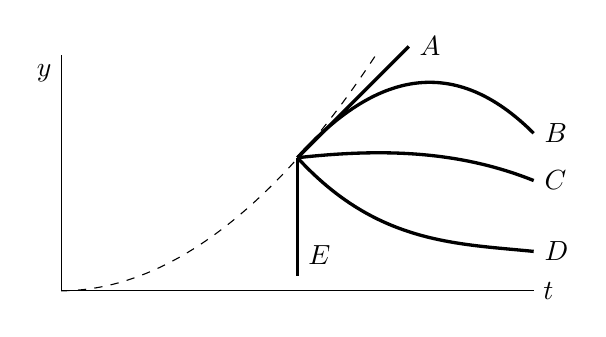
\begin{tikzpicture}
        %% Axis
        \draw (0,0) -- (6,0) node[anchor=west] {$t$};
        \draw (0,0) -- (0,3) node[anchor=north east] {$y$};
        %% parabola
        \draw[dashed] (0,0) parabola bend (0,0) (4,3);
        %% Options
        \draw[very thick] (3,1.69) -- ++(45:2) node[anchor=west] {$A$};
        \draw[very thick] (3,1.69) -- ++(270:1.5) node[anchor=south west] {$E$};
        \draw[very thick] (3,1.69) .. controls (4,2.8) and (5,3.0) .. (6,2.0) node[anchor=west] {$B$};
        \draw[very thick] (3,1.69) .. controls (4,1.8) and (5,1.8) .. (6,1.4) node[anchor=west] {$C$};
        \draw[very thick] (3,1.69) .. controls (4,0.6) and (5,0.6) .. (6,0.5) node[anchor=west] {$D$};
    \end{tikzpicture}
    \end{center}
    At the instant indicated by the dot,
        a bolt breaks loose and drops from the ceiling. 
    Which curve best represents the position of the bolt as a function of time?
    \begin{multicols}{5}
    \begin{choices}[o]
        \wrongchoice{$A$}
      \correctchoice{$B$}
        \wrongchoice{$C$}
        \wrongchoice{$D$}
        \wrongchoice{$E$}
    \end{choices}
\end{multicols}
\end{question}
}

\element{halliday-mc}{
\begin{question}{halliday-ch02-q70}
    The diagram shows a velocity-time graph for a car moving in a straight line. 
    \begin{center}
    \begin{tikzpicture}
        \draw (0,-1) -- (0,3) node[anchor=east] {$v$};
        \draw (0,0) -- (5,0) node[anchor=west] {$t$};
        \draw[very thick] (0,0) .. controls (2,4) and (4,2) .. (5,-0.8)
            node[pos=0.3,anchor=south east] {$P$}
            node[pos=0.3,circle,draw,thin,minimum size=2pt] {}
            node[pos=0.95,anchor=north east] {$Q$}
            node[pos=0.95,circle,draw,thin,minimum size=2pt] {};
    \end{tikzpicture}
    \end{center}
    At point $Q$ the car must be:
    \begin{choices}
        \wrongchoice{moving with zero acceleration}
        \wrongchoice{traveling downhill}
        \wrongchoice{traveling below ground-level}
        \wrongchoice{reducing speed}
      \correctchoice{traveling in the reverse direction to that at point P}
    \end{choices}
\end{question}
}

\element{halliday-mc}{
\begin{question}{halliday-ch02-q71}
    The diagram shows a velocity-time graph for a car moving in a straight line. 
    \begin{center}
    \begin{tikzpicture}
        \draw (0,-1) -- (0,3) node[anchor=east] {$v$};
        \draw (0,0) -- (5,0) node[anchor=west] {$t$};
        \draw[very thick] (0,0) .. controls (3,3) and (4,3) .. (5,3)
            node[pos=0.25,anchor=south east] {$P$}
            node[pos=0.25,circle,draw,thin,minimum size=2pt] {};
    \end{tikzpicture}
    \end{center}
    At point $P$ the car must be:
    \begin{choices}
        \wrongchoice{moving with zero acceleration}
        \wrongchoice{climbing the hill}
      \correctchoice{accelerating}
        \wrongchoice{stationary}
        \wrongchoice{moving at about \ang{45} with respect to the $x$ axis}
    \end{choices}
\end{question}
}

\newcommand{\hallidayChTwoQSeventyTwo}{
\begin{tikzpicture}
    \begin{axis}[
        axis y line=left, 
        axis x line=bottom, 
        axis line style={->},
        xlabel={time},
        x unit=\si{\second},
        xtick={0,2,5,9},
        ylabel={velocity},
        y unit=\si{\meter\per\second},
        ytick={0,6,12},
        grid=major,
        xmin=0,xmax=10,
        ymin=0,ymax=13,
        width=0.95\columnwidth,
        height=0.50\columnwidth,
    ]
    \addplot[line width=1pt,mark=\empty] plot coordinates { (0,0) (2,12) (5,12) (9,0) };
    \end{axis}
\end{tikzpicture}
}

\element{halliday-mc}{
\begin{question}{halliday-ch02-q72}
    The graph represents the straight line motion of a car. 
    \begin{center}
        \hallidayChTwoQSeventyTwo
    \end{center}
    How far does the car travel between $t=\SI{2}{\second}$ and $t=\SI{5}{\second}$?
    \begin{multicols}{3}
    \begin{choices}
        \wrongchoice{\SI{4}{\meter}}
        \wrongchoice{\SI{12}{\meter}}
        \wrongchoice{\SI{24}{\meter}}
      \correctchoice{\SI{36}{\meter}}
        \wrongchoice{\SI{60}{\meter}}
        %% Added for Symmetry
        \wrongchoice{\SI{0}{\meter}}
    \end{choices}
    \end{multicols}
\end{question}
}

\element{halliday-mc}{
\begin{question}{halliday-ch02-q73}
    The diagram represents the straight line motion of a car. 
    \begin{center}
        \hallidayChTwoQSeventyTwo
    \end{center}
    Which of the following statements is true?
    \begin{choices}
        \wrongchoice{The car accelerates, stops, and reverses}
      \correctchoice{The car accelerates at \SI{6}{\meter\per\second\squared} for the first \SI{2}{\second}}
        \wrongchoice{The car is moving for a total time of \SI{12}{\second}}
        \wrongchoice{The car decelerates at \SI{12}{\meter\per\second\squared} for the last \SI{4}{\second}}
        \wrongchoice{The car returns to its starting point when $t=\SI{9}{\second}$}
    \end{choices}
\end{question}
}

\element{halliday-mc}{
\begin{questionmult}{halliday-ch02-q74}
    %Consider the following five graphs (note the axes carefully). 
    Consider the following six graphs (note the axes carefully). 
    Which of these represents motion at constant speed?
    \begin{multicols}{2}
    \begin{choices}
        \AMCboxDimensions{down=-2.5em}
        %% ANS is E: I and IV only
        \correctchoice{
            \begin{tikzpicture}
                \begin{axis}[
                    axis y line=left,
                    axis x line=bottom,
                    axis line style={->},
                    xlabel={time},
                    xtick=\empty,
                    ylabel={position},
                    ytick=\empty,
                    xmin=0,xmax=11,
                    ymin=0,ymax=11,
                    width=0.95\columnwidth,
                    very thin,
                ]
                \addplot[line width=1pt,mark=\empty] plot coordinates { (0,0) (10,10) };
                \end{axis}
            \end{tikzpicture}
        }
        %% II
        \wrongchoice{
            \begin{tikzpicture}
                \begin{axis}[
                    axis y line=left,
                    axis x line=bottom,
                    axis line style={->},
                    xlabel={time},
                    xtick=\empty,
                    ylabel={velocity},
                    ytick=\empty,
                    xmin=0,xmax=11,
                    ymin=0,ymax=11,
                    width=0.95\columnwidth,
                    very thin,
                ]
                \addplot[line width=1pt,mark=\empty] plot coordinates { (0,0) (10,10) };
                \end{axis}
            \end{tikzpicture}
        }
        %% III
        \wrongchoice{
            \begin{tikzpicture}
                \begin{axis}[
                    axis y line=left,
                    axis x line=bottom,
                    axis line style={->},
                    xlabel={time},
                    xtick=\empty,
                    ylabel={acceleration},
                    ytick=\empty,
                    xmin=0,xmax=11,
                    ymin=0,ymax=11,
                    width=0.95\columnwidth,
                    very thin,
                ]
                \addplot[line width=1pt,mark=\empty] plot coordinates { (0,0) (10,10) };
                \end{axis}
            \end{tikzpicture}
        }
        %% ANS is E: I and IV only
        \correctchoice{
            \begin{tikzpicture}
                \begin{axis}[
                    axis y line=left,
                    axis x line=bottom,
                    axis line style={->},
                    xlabel={time},
                    xtick=\empty,
                    ylabel={velocity},
                    ytick=\empty,
                    xmin=0,xmax=11,
                    ymin=0,ymax=11,
                    width=0.95\columnwidth,
                    very thin,
                ]
                \addplot[line width=1pt,mark=\empty] plot coordinates { (0,8) (10,8) };
                \end{axis}
            \end{tikzpicture}
        }
        %% V
        \wrongchoice{
            \begin{tikzpicture}
                \begin{axis}[
                    axis y line=left,
                    axis x line=bottom,
                    axis line style={->},
                    xlabel={time},
                    xtick=\empty,
                    ylabel={acceleration},
                    ytick=\empty,
                    xmin=0,xmax=11,
                    ymin=0,ymax=11,
                    width=0.95\columnwidth,
                    very thin,
                ]
                \addplot[line width=1pt,mark=\empty] plot coordinates { (0,8) (10,8) };
                \end{axis}
            \end{tikzpicture}
        }
        %% Added for Symmetry
        \wrongchoice{
            \begin{tikzpicture}
                \begin{axis}[
                    axis y line=left,
                    axis x line=bottom,
                    axis line style={->},
                    xlabel={time},
                    xtick=\empty,
                    ylabel={position},
                    ytick=\empty,
                    xmin=0,xmax=11,
                    ymin=0,ymax=11,
                    width=0.95\columnwidth,
                    very thin,
                ]
                \addplot[line width=1pt,domain=0:10] {0.1*x*x};
                \end{axis}
            \end{tikzpicture}
        }
    \end{choices}
    \end{multicols}
\end{questionmult}
}

\element{halliday-mc}{
\begin{question}{halliday-ch02-q75}
    An object is dropped from rest. 
    %Which of the following five graphs correctly represents its motion? 
    Which of the following six graphs correctly represents its motion? 
    The positive direction is taken to be downward.
    \begin{multicols}{2}
    \begin{choices}
        \AMCboxDimensions{down=-2.5em}
        \wrongchoice{
            \begin{tikzpicture}
                \begin{axis}[
                    axis y line=left,
                    axis x line=bottom,
                    axis line style={->},
                    xlabel={time},
                    xtick=\empty,
                    ylabel={velocity},
                    ytick=\empty,
                    xmin=0,xmax=11,
                    ymin=0,ymax=11,
                    width=0.95\columnwidth,
                    very thin,
                ]
                \addplot[line width=1pt,mark=\empty] plot coordinates { (0,8) (10,8) };
                \end{axis}
            \end{tikzpicture}
        }
        %% ANS is B
        \correctchoice{
            \begin{tikzpicture}
                \begin{axis}[
                    axis y line=left,
                    axis x line=bottom,
                    axis line style={->},
                    xlabel={time},
                    xtick=\empty,
                    ylabel={velocity},
                    ytick=\empty,
                    xmin=0,xmax=11,
                    ymin=0,ymax=11,
                    width=0.95\columnwidth,
                    very thin,
                ]
                \addplot[line width=1pt,mark=\empty] plot coordinates { (0,0) (10,10) };
                \end{axis}
            \end{tikzpicture}
        }
        \wrongchoice{
            \begin{tikzpicture}
                \begin{axis}[
                    axis y line=left,
                    axis x line=bottom,
                    axis line style={->},
                    xlabel={time},
                    xtick=\empty,
                    ylabel={velocity},
                    ytick=\empty,
                    xmin=0,xmax=11,
                    ymin=0,ymax=11,
                    width=0.95\columnwidth,
                    very thin,
                ]
                \addplot[line width=1pt,domain=0:10]{0.1*x*x};
                \end{axis}
            \end{tikzpicture}
        }
        \wrongchoice{
            \begin{tikzpicture}
                \begin{axis}[
                    axis y line=left,
                    axis x line=bottom,
                    axis line style={->},
                    xlabel={time},
                    xtick=\empty,
                    ylabel={velocity},
                    ytick=\empty,
                    xmin=0,xmax=11,
                    ymin=0,ymax=11,
                    width=0.95\columnwidth,
                    very thin,
                ]
                \addplot[line width=1pt,domain=0:10]{10 - 0.1*(x-10)*(x-10)};
                \end{axis}
            \end{tikzpicture}
        }
        \wrongchoice{
            \begin{tikzpicture}
                \begin{axis}[
                    axis y line=left,
                    axis x line=bottom,
                    axis line style={->},
                    xlabel={time},
                    xtick=\empty,
                    ylabel={height},
                    ytick=\empty,
                    xmin=0,xmax=11,
                    ymin=0,ymax=11,
                    width=0.95\columnwidth,
                    very thin,
                ]
                \addplot[line width=1pt,domain=0:10]{10 - 0.4*(x-5)*(x-5)};
                \end{axis}
            \end{tikzpicture}
        }
        %% Added for Symmetry
        \wrongchoice{
            \begin{tikzpicture}
                \begin{axis}[
                    axis y line=left,
                    axis x line=middle,
                    axis line style={->},
                    xlabel={time},
                    xtick=\empty,
                    ylabel={velocity},
                    ytick=\empty,
                    xmin=0,xmax=11,
                    ymin=-6,ymax=6,
                    width=0.95\columnwidth,
                    very thin,
                ]
                \addplot[line width=1pt,mark=\empty] plot coordinates { (0,5) (10,-5) };
                \end{axis}
            \end{tikzpicture}
        }
    \end{choices}
    \end{multicols}
\end{question}
}

\element{halliday-mc}{
\begin{question}{halliday-ch02-q76}
    A stone is dropped from a cliff. 
    The graph (carefully note the axes) which best represents its motion while it falls
    \begin{multicols}{2}
    \begin{choices}
        \AMCboxDimensions{down=-2.5em}
        \wrongchoice{
            \begin{tikzpicture}
                \begin{axis}[
                    axis y line=left,
                    axis x line=bottom,
                    axis line style={->},
                    xlabel={time},
                    xtick=\empty,
                    ylabel={position},
                    ytick=\empty,
                    xmin=0,xmax=11,
                    ymin=0,ymax=11,
                    width=0.95\columnwidth,
                    very thin,
                ]
                \addplot[line width=1pt,domain=0:10]{x};
                \end{axis}
            \end{tikzpicture}
        }
        \wrongchoice{
            \begin{tikzpicture}
                \begin{axis}[
                    axis y line=left,
                    axis x line=bottom,
                    axis line style={->},
                    xlabel={time},
                    xtick=\empty,
                    ylabel={velocity},
                    ytick=\empty,
                    xmin=0,xmax=11,
                    ymin=0,ymax=11,
                    width=0.95\columnwidth,
                    very thin,
                ]
                \addplot[line width=1pt,domain=0:10]{0.1*x*x};
                \end{axis}
            \end{tikzpicture}
        }
        %% ANS is C
        \correctchoice{
            \begin{tikzpicture}
                \begin{axis}[
                    axis y line=left,
                    axis x line=bottom,
                    axis line style={->},
                    xlabel={time},
                    xtick=\empty,
                    ylabel={velocity},
                    ytick=\empty,
                    xmin=0,xmax=11,
                    ymin=0,ymax=11,
                    width=0.95\columnwidth,
                    very thin,
                ]
                \addplot[line width=1pt,domain=0:10]{x};
                \end{axis}
            \end{tikzpicture}
        }
        \wrongchoice{
            \begin{tikzpicture}
                \begin{axis}[
                    axis y line=left,
                    axis x line=bottom,
                    axis line style={->},
                    xlabel={time},
                    xtick=\empty,
                    ylabel={acceleration},
                    ytick=\empty,
                    xmin=0,xmax=11,
                    ymin=0,ymax=11,
                    width=0.95\columnwidth,
                    very thin,
                ]
                \addplot[line width=1pt,domain=0:10]{0.1*x*x};
                \end{axis}
            \end{tikzpicture}
        }
        \wrongchoice{
            \begin{tikzpicture}
                \begin{axis}[
                    axis y line=left,
                    axis x line=bottom,
                    axis line style={->},
                    xlabel={time},
                    xtick=\empty,
                    ylabel={acceleration},
                    ytick=\empty,
                    xmin=0,xmax=11,
                    ymin=0,ymax=11,
                    width=0.95\columnwidth,
                    very thin,
                ]
                \addplot[line width=1pt,domain=0:10]{x};
                \end{axis}
            \end{tikzpicture}
        }
        %% Added for Symmetry
        \wrongchoice{
            \begin{tikzpicture}
                \begin{axis}[
                    axis y line=left,
                    axis x line=bottom,
                    axis line style={->},
                    xlabel={time},
                    xtick=\empty,
                    ylabel={velocity},
                    ytick=\empty,
                    xmin=0,xmax=11,
                    ymin=0,ymax=11,
                    width=0.95\columnwidth,
                    very thin,
                ]
                \addplot[line width=1pt,mark=\empty] plot coordinates { (0,8) (10,8) };
                \end{axis}
            \end{tikzpicture}
        }
    \end{choices}
    \end{multicols}
\end{question}
}

\element{halliday-mc}{
\begin{question}{halliday-ch02-q77}
    An object is thrown vertically into the air. 
    %Which of the following five graphs represents the velocity ($v$) of the object as a function of the time ($t$)? 
    Which of the following six graphs represents the velocity of the object as a function of the time? 
    The positive direction is taken to be upward.
    \begin{multicols}{2}
    \begin{choices}
        \AMCboxDimensions{down=-2.5em}
        \wrongchoice{
            \begin{tikzpicture}
                \begin{axis}[
                    axis y line=left,
                    axis x line=bottom,
                    axis line style={->},
                    xlabel={time},
                    xtick=\empty,
                    ylabel={velocity},
                    ytick=\empty,
                    xmin=0,xmax=11,
                    ymin=0,ymax=11,
                    width=0.95\columnwidth,
                    very thin,
                ]
                \addplot[line width=1pt,domain=0:10]{x};
                \end{axis}
            \end{tikzpicture}
        }
        \wrongchoice{
            \begin{tikzpicture}
                \begin{axis}[
                    axis y line=left,
                    axis x line=bottom,
                    axis line style={->},
                    xlabel={time},
                    xtick=\empty,
                    ylabel={velocity},
                    ytick=\empty,
                    xmin=0,xmax=11,
                    ymin=0,ymax=11,
                    width=0.95\columnwidth,
                    very thin,
                ]
                \addplot[line width=1pt,domain=0:10]{8};
                \end{axis}
            \end{tikzpicture}
        }
        %% ANS is C
        \correctchoice{
            \begin{tikzpicture}
                \begin{axis}[
                    axis y line=left,
                    axis x line=middle,
                    axis line style={->},
                    xlabel={time},
                    xtick=\empty,
                    ylabel={velocity},
                    ytick=\empty,
                    xmin=0,xmax=11,
                    ymin=-6,ymax=6,
                    width=0.95\columnwidth,
                    very thin,
                ]
                \addplot[line width=1pt,domain=0:10]{5-x};
                \end{axis}
            \end{tikzpicture}
        }
        \wrongchoice{
            \begin{tikzpicture}
                \begin{axis}[
                    axis y line=left,
                    axis x line=bottom,
                    axis line style={->},
                    xlabel={time},
                    xtick=\empty,
                    ylabel={velocity},
                    ytick=\empty,
                    xmin=0,xmax=11,
                    ymin=0,ymax=11,
                    width=0.95\columnwidth,
                    very thin,
                ]
                \addplot[line width=1pt,domain=0:10]{0.1*x*x};
                \end{axis}
            \end{tikzpicture}
        }
        \wrongchoice{
            \begin{tikzpicture}
                \begin{axis}[
                    axis y line=left,
                    axis x line=bottom,
                    axis line style={->},
                    xlabel={time},
                    xtick=\empty,
                    ylabel={velocity},
                    ytick=\empty,
                    xmin=0,xmax=11,
                    ymin=0,ymax=11,
                    width=0.95\columnwidth,
                    very thin,
                ]
                \addplot[line width=1pt,domain=0:10]{10-0.1*(x-10)*(x-10)};
                \end{axis}
            \end{tikzpicture}
        }
        %% Added for Symmetry
        \wrongchoice{
            \begin{tikzpicture}
                \begin{axis}[
                    axis y line=left,
                    axis x line=middle,
                    axis line style={->},
                    xlabel={time},
                    x label style={
                        anchor=north east,
                    },
                    xtick=\empty,
                    ylabel={velocity},
                    ytick=\empty,
                    xmin=0,xmax=11,
                    ymin=-6,ymax=6,
                    width=0.95\columnwidth,
                    very thin,
                ]
                \addplot[line width=1pt,domain=0:10]{-5+x};
                \end{axis}
            \end{tikzpicture}
        }
    \end{choices}
    \end{multicols}
\end{question}
}


\endinput


